This section shows the results obtained with the TRITIUM-IFIC 1 prototype  during its installation in the Nuclear Radiation Laboratory at IFIC. Its design is explained in section \ref{subsec:TritiumIFIC1}, which includes several improvements, such as a Teflon vessel and new straight arrangement of scintillating fibers, which were found to be a problems in the previous prototype, reducing its efficiency.

The energy spectra of both, signal and background, were measured with TRITIUM-IFIC 1 prototype, which is shown in Figure \ref{subfig:SignalBackgroundEnergySpectraTritiumIFIC1}. As it was mentioned in section \ref{subsec:TritiumIFIC1}, to mesure the signal, the prototype was filled with a tritiated water solution with an activity of $99.696~\kilo\becquerel/\liter$ and, to measure the background, the prototype was filled with ultrapure water.

\begin{figure}
\centering
    \begin{subfigure}[b]{1\textwidth}
    \centering
    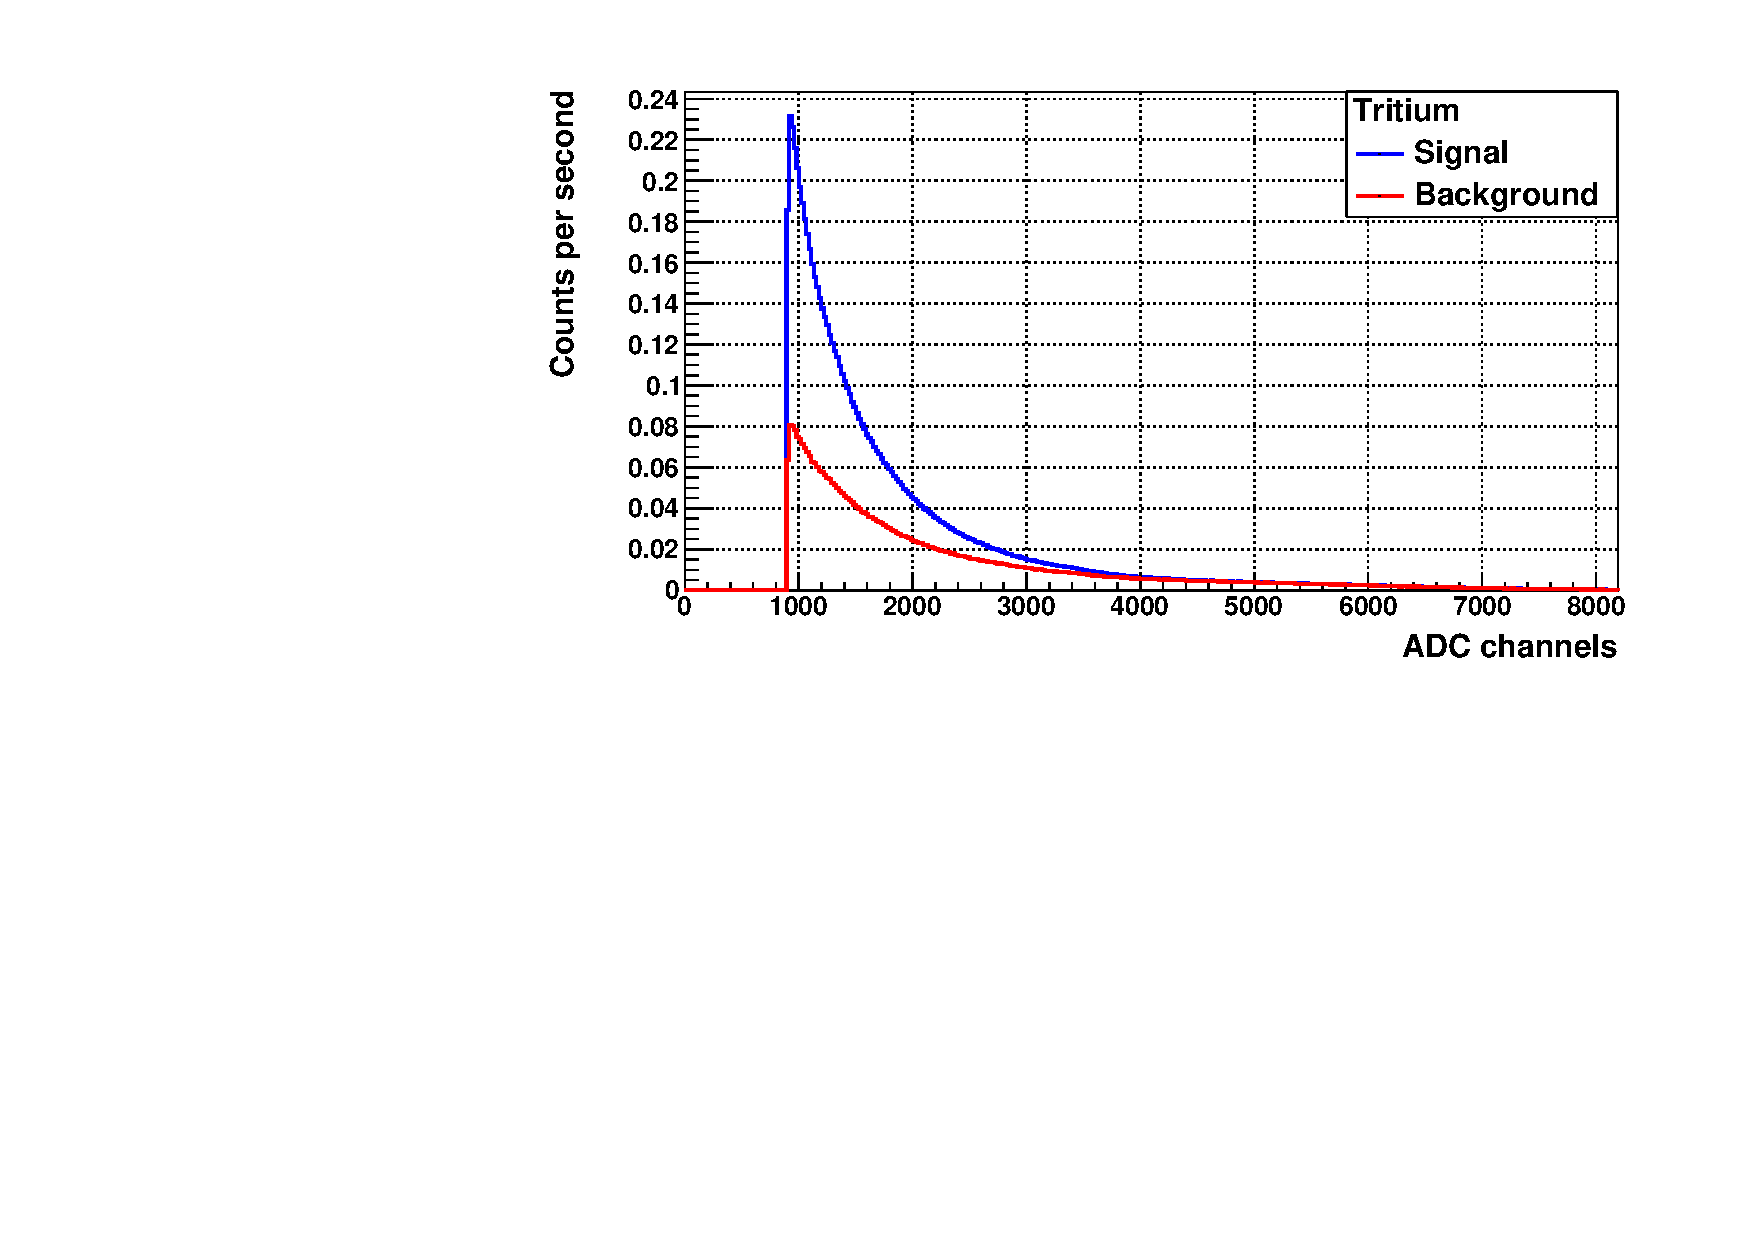
\includegraphics[width=\textwidth]{7ExperimentalResultsDetectors/71ExperimentalResultsLaboratory/712TRITIUMIFIC1/TritiumIFIC1Signals.pdf}  
    \caption{\label{subfig:SignalBackgroundEnergySpectraTritiumIFIC1}}
    \end{subfigure}
    \hfill
    \begin{subfigure}[b]{1\textwidth}
    \centering
    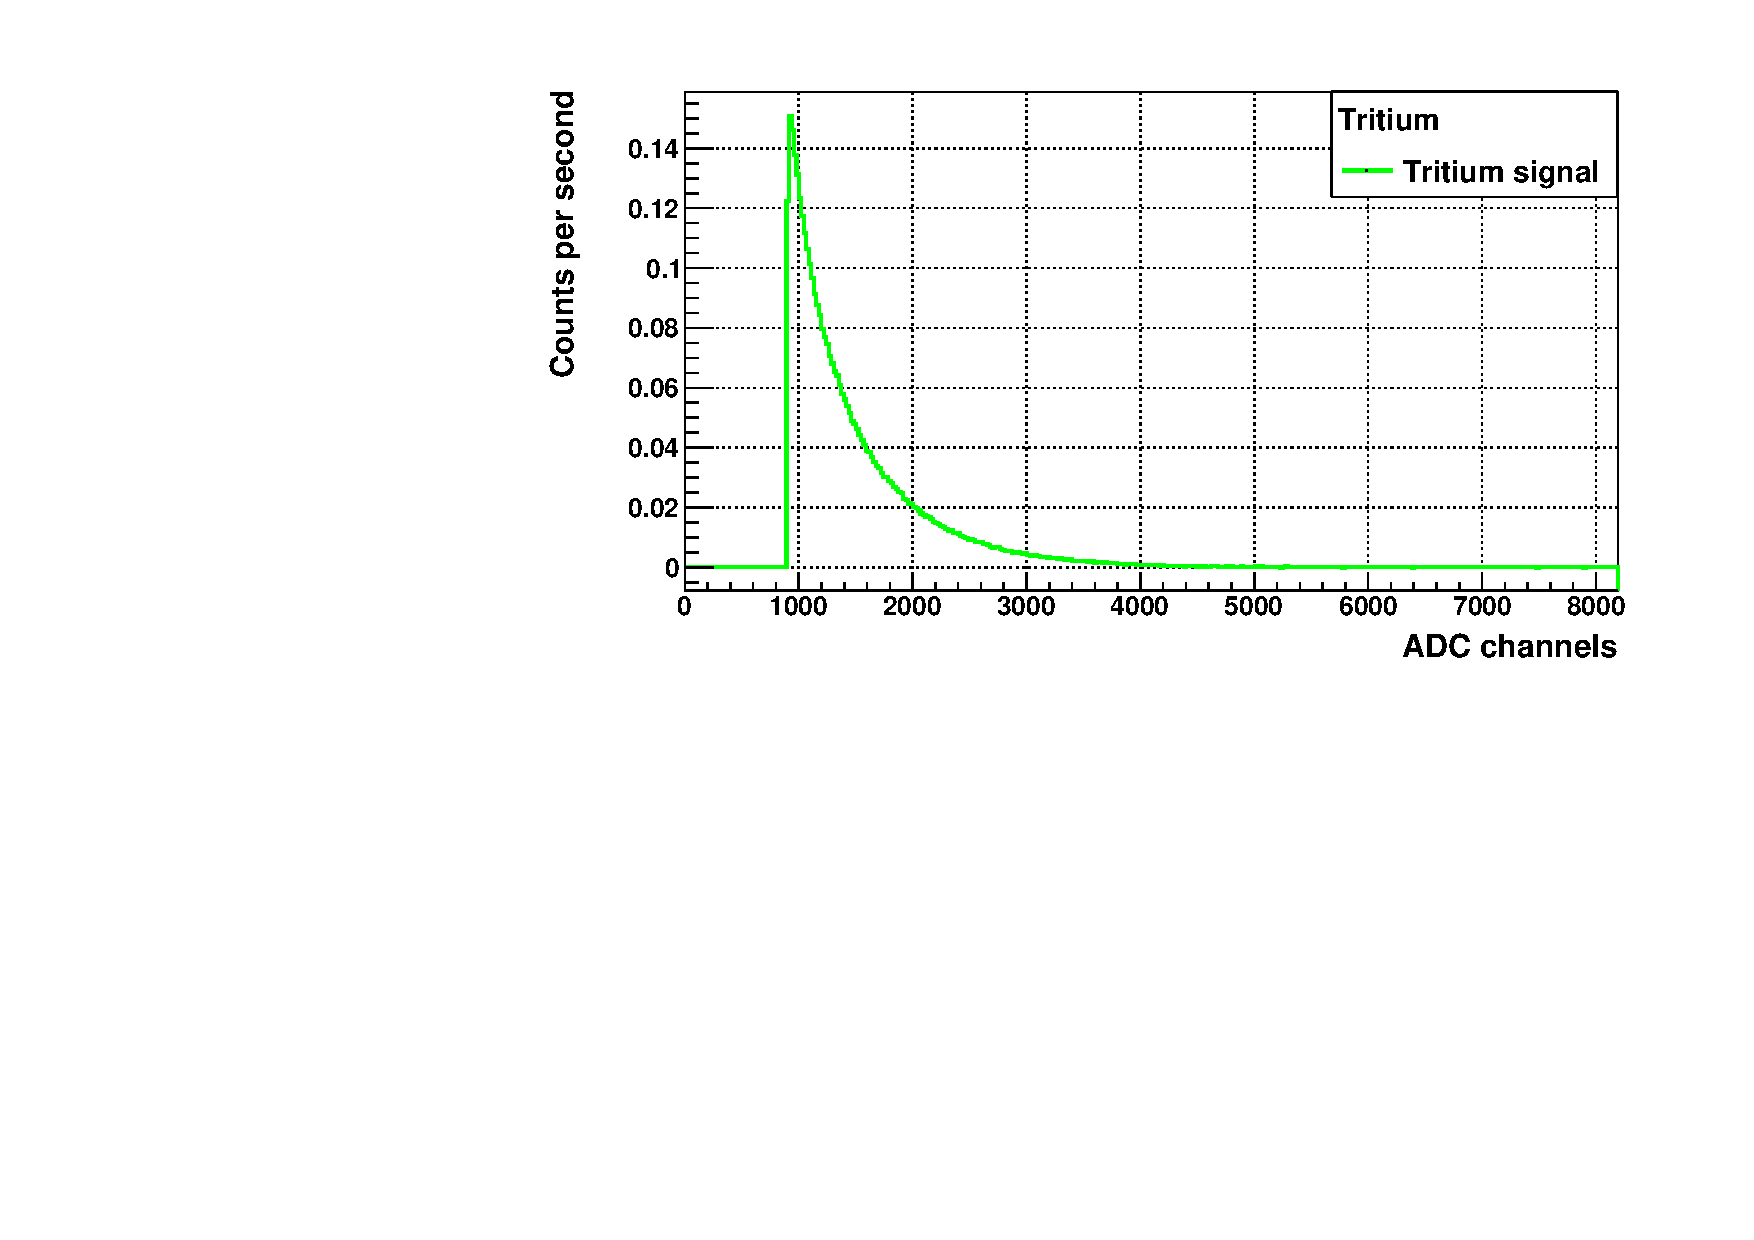
\includegraphics[width=\textwidth]{7ExperimentalResultsDetectors/71ExperimentalResultsLaboratory/712TRITIUMIFIC1/TritiumIFIC1Clear.pdf}  
    \caption{\label{subfig:TritiumEnergySpectraTritiumIFIC1}}
    \end{subfigure}
 \caption{Energy spectra experimentally measured with TRITIUM-IFIC 1 prototype. Above) Signal and background energy spectra. Below) Tritium energy spectrum.}
 \label{fig:EnergySpectraTRITIUMIFIC1}
\end{figure}

%\begin{figure}[htbp]
%\centering
%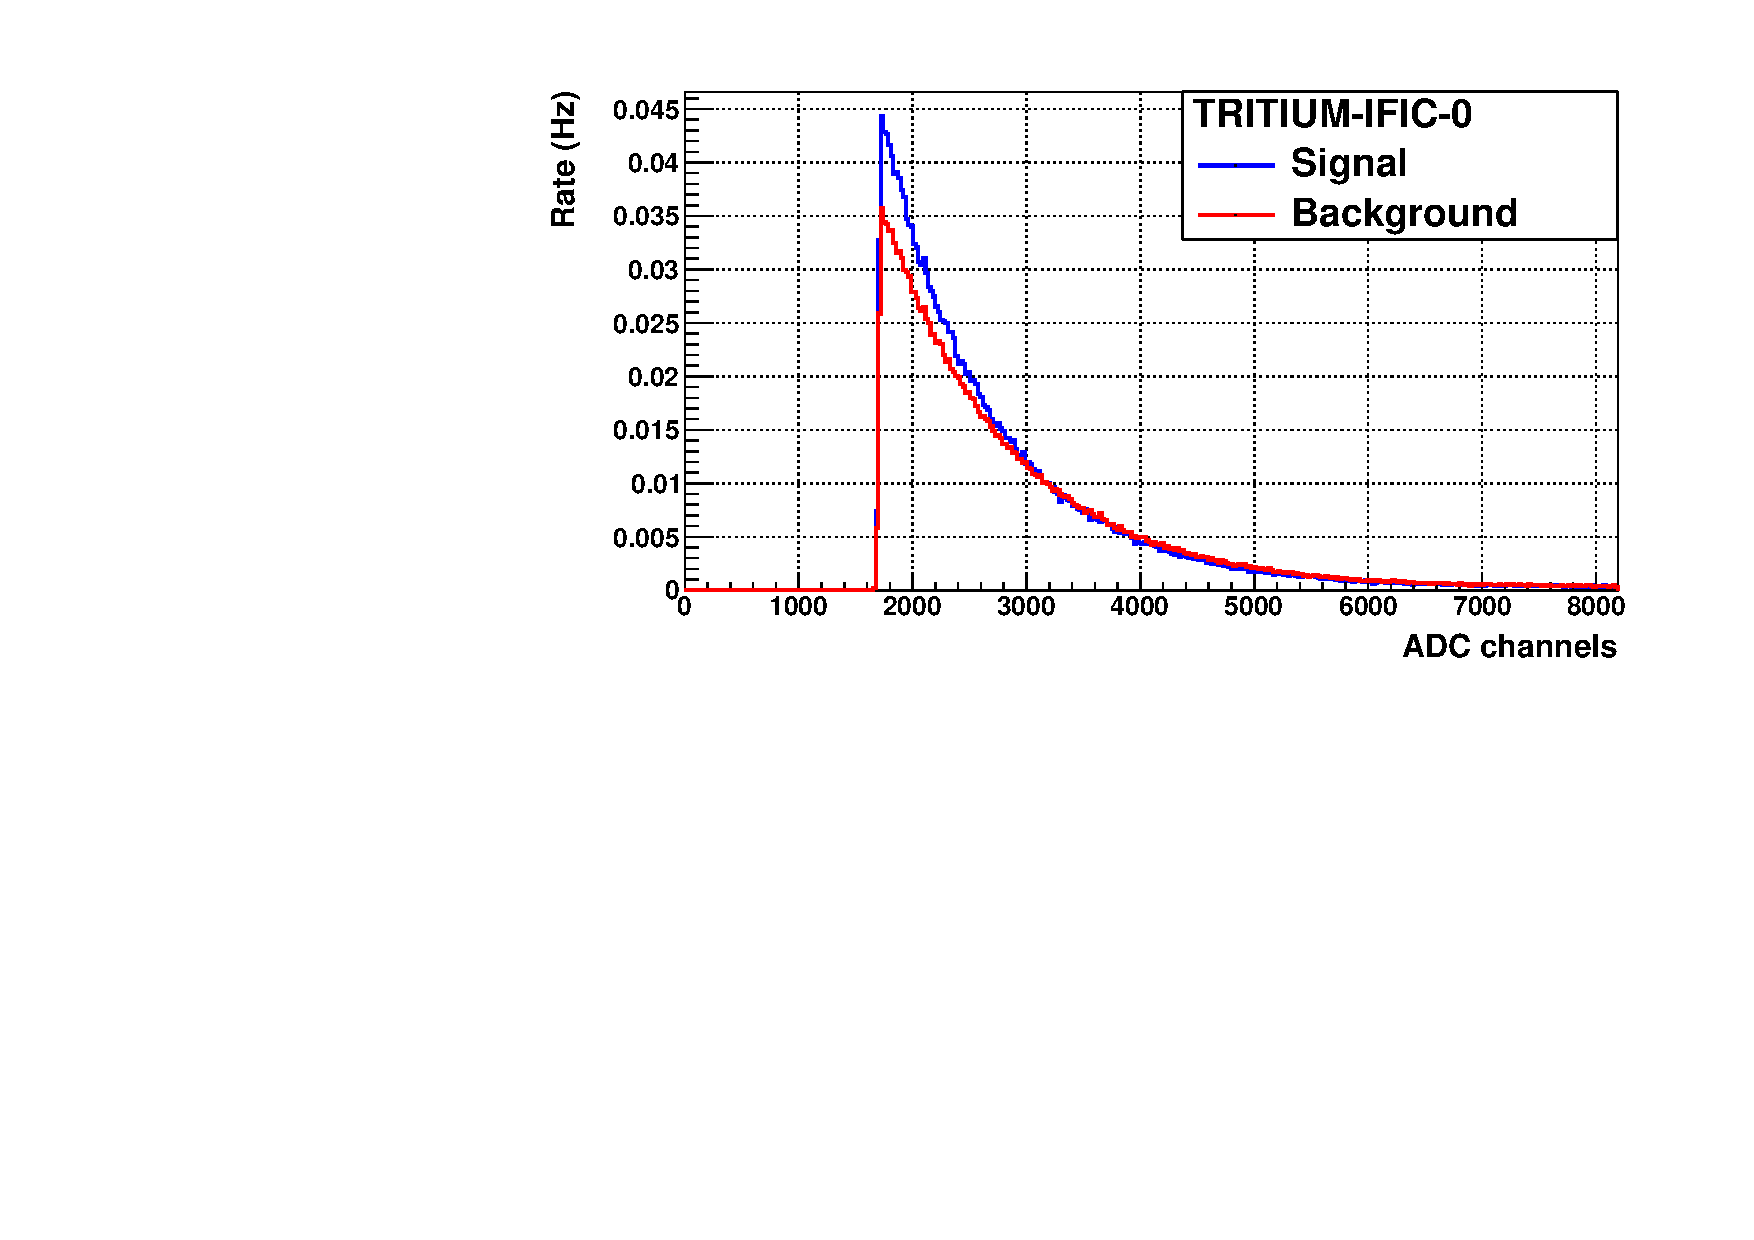
\includegraphics[scale=0.6]{7ExperimentalResultsDetectors/71ExperimentalResultsLaboratory/711TritiumIFIC0/TritiumIFIC0Signals.pdf}
%\caption{Energy spectra experimentally measured with TRITIUM-IFIC 0 prototype.).\label{fig:EnergySpectrumTritiumIFIC0}}
%\end{figure}

As can be see, the difference between both energy spectra is clearly visible, which corresponds to the trtium energy spectrum, Figura \ref{subfig:TritiumEnergySpectraTritiumIFIC1}. Furthermore, compared to the energy spectra obtained with the previous prototype, Figure \ref{subfig:SignalBackgroundEnergySpectraTritiumIFIC0}, the difference between both is larger, which implies that the tritium detection efficiency of this prototype was improved.

This efficiency improvement can be quantified using similar calculations than the previous section. The number of counts per second measured for these three signals are shown in Table \ref{tab:CountsPerSecondTRITIUMIFIC1}, where the tritium counts was obtained from the difference of signal and background.

\begin{table}[h]
%%\centering
\begin{center}
\begin{tabular}{|c|c|}
\hline
Spectrum & Counts/second\\
\hline \hline \hline
Signal prototype & $7.82 \pm 0.11$ \\ \hline
Background prototype & $3.99 \pm 0.08$ \\ \hline
Tritium counts & $3.83 \pm 0.13$ \\ \hline
\end{tabular}
\caption{Counts per second obtained with TRITIUM-IFIC 1 prototype.}
\label{tab:CountsPerSecondTRITIUMIFIC1}
\end{center}
\end{table}

The tritium detection efficiency obtained for TRITIUM-IFIC 1 is $(3.84 \pm 0.16)\cdot{} 10^{-2}~ \frac{\text{c}/\second}{\kilo\becquerel/\liter}$, which is calculated using the same quotient explained in the previous section. As can be seen, the efficiency obtained for this prototype is larger than that obtained for the previous prototype, TRITIUM-IFIC 0. It is an expected result since this prototype uses a larger active area. The specific efficiency is calculated to eliminate the effect this different between both prototypes and quantify the improvement in the efficiency due to modifications in the design. The specific efficiency obtained is $(9.56 \pm 0.40)\cdot{} 10^{-5}~ \frac{\text{c}/\second}{\kilo\becquerel/\liter}\frac{1}{\cm^{2}}$.

Therefore it was verified that the specific efficiency of this prototype was improved by a factor of ten due to the modifications applied to its design which confirms and quantifies the usefulness of these modifications. Furthermore, compared with scintillating detectors developed in other experiments, table \ref{tab:PlasticScinTritium}, on the one hand, the efficiency of this prototype is very close to the best result, obtained for Singh, and, on the other hand, the specific efficiency, which is the most relevant value to compare, is almost 5 times larger than the best results, obtained for Hofstetter.

It must be taken into account that in the first two prototypes the Low Detection Level, LDL, was not studied, since their objective was to improve its design and find the problems that reduced their efficiency. In fact, it can be seen in Figure \ref{fig:EnergySpectraTRITIUMIFIC1} that the activity used is further to be the LDL of the TRITIUM-IFIC 1 prototype. The LDL was only studied in the final prototypes.